\documentclass[14pt, aspectratio=169]{beamer}

\usetheme{Copenhagen}
\setbeamertemplate{navigation symbols}{} % Esconde as barras de navegação inferiores
\setbeamercovered{transparent}
\setbeamertemplate{headline}{} % Esconde a barra de navegação no topo do documento, relativa às seções
\setbeamertemplate{caption}[numbered] % Coloca os números nas figuras

\newcommand{\C}{\mathbb{C}}
\newcommand{\R}{\mathbb{R}}
\newcommand{\I}{\mathbb{I}}
\newcommand{\Q}{\mathbb{Q}}
\newcommand{\Z}{\mathbb{Z}}
\newcommand{\N}{\mathbb{N}}

\newcommand{\conj}[1]{\left\{ #1 \right\}}
\newcommand{\skipframe}{\vspace{10.0cm}}
\newcommand{\parenthesis}[1]{\left( #1 \right)}

\newtheorem{theo}{Teorema}
\newtheorem{ex}{Exemplo}

\input{pacotes.tex}

\title{Funções}
\subtitle{Pré-cálculo}
\author{Prof. Dr. Márcio Leandro Gonçalves}
\date{\today}
\institute{PUC Minas - Poços de Caldas}

\begin{document}

\begin{frame}
\maketitle 
\end{frame}

\begin{frame}{Sumário}
    \begin{multicols}{2}
        \tableofcontents
    \end{multicols}
\end{frame}

\section{Conceitos iniciais}

\begin{frame}[allowframebreaks]{Conceitos iniciais}

\begin{itemize}
    \item Função: é uma regra ou lei que associa cada elemento de um conjunto um único elemento de outro conjunto.

    \vspace{0.5cm}

    \begin{multicols}{2}
        \begin{figure}
        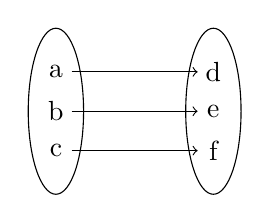
\begin{tikzpicture}
            \draw (0,0) ellipse (10pt and 30pt);
            \draw (2,0) ellipse (10pt and 30pt);

            \draw node at (0, 0.5) {a};
            \draw node at (0, 0) {b};
            \draw node at (0, -0.5) {c};

            \draw node at (2, 0.5) {d};
            \draw node at (2, 0) {e};
            \draw node at (2, -0.5) {f};

            \draw [->] (0 + 0.2, 0.5) -- (2 - 0.2, 0.5);
            \draw [->] (0 + 0.2, 0) -- (2 - 0.2, 0);
            \draw [->] (0 + 0.2, -0.5) -- (2 - 0.2, -0.5);
    \end{tikzpicture}
    \caption{É função}
    \end{figure}

    \begin{figure}
        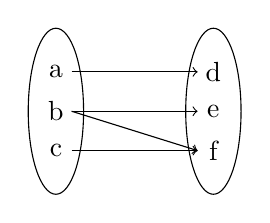
\begin{tikzpicture}
            \draw (0,0) ellipse (10pt and 30pt);
            \draw (2,0) ellipse (10pt and 30pt);

            \draw node at (0, 0.5) {a};
            \draw node at (0, 0) {b};
            \draw node at (0, -0.5) {c};

            \draw node at (2, 0.5) {d};
            \draw node at (2, 0) {e};
            \draw node at (2, -0.5) {f};

            \draw [->] (0 + 0.2, 0.5) -- (2 - 0.2, 0.5);
            \draw [->] (0 + 0.2, 0) -- (2 - 0.2, 0);
            \draw [->] (0 + 0.2, 0) -- (2 - 0.2, -0.5);
            \draw [->] (0 + 0.2, -0.5) -- (2 - 0.2, -0.5);
    \end{tikzpicture}
    \caption{Não é função}
    \end{figure}
    \end{multicols}

    \skipframe

    \item De forma prática, pode-se ver, através de um gráfico, se uma relação é uma função pelo \emph{teste da reta vertical}.

    \item O teste consiste em traçar retas verticais por pontos do eixo $x$ (domínio) e, se ela cortar o gráfico em mais de um ponto, esta relação não representa uma função.

    \skipframe

    \begin{figure}
        \centering
        \begin{tikzpicture}[scale=0.8]
        \draw[color=blue] (3.43,2.85) circle (1);
        \draw[color=red] (2.8, 5) -- (2.8, 1);
        \begin{axis}[xmin=-5, xmax=5, ymin=-5, ymax=5, axis lines=middle]
        \end{axis}
        \end{tikzpicture}
        \caption{Não é função}
    \end{figure}

    \skipframe

    \item O método mais comum de visualizar uma função consiste em fazer seu gráfico. 

    \item Dada uma função $f:A \rightarrow B$, o gráfico de $f$ será o conjunto de pares ordenados $G(f) = \conj{(x, f(x)) \mid x \in A}$.

    \skipframe

    \begin{figure}
        \centering
        \begin{tikzpicture}[scale=0.8]
        \begin{axis}[xmin=-5, xmax=5, ymin=-5, ymax=5, axis lines=middle]
            \addplot{(x - 2)^2 - 3};
        \end{axis}
        \end{tikzpicture}
        \caption{$f(x) = (x - 2)^2 - 3$}
    \end{figure}

    \skipframe

    \item Dada uma função $f:A \rightarrow B$, define-se, informalmente:

    \begin{itemize}
         \item Domínio ($A$ ou $D(f)$): conjunto de todos os valores possíveis de substituírem a variável na função. 

        \item Imagem ($Im(f)$): conjunto de todos os valores a serem retornados da função, ou seja, todos of valores de $f(x)$ quando $x$ varia em $D(f)$.

        \item Contradomínio ($B$ ou $CD(f)$): conjunto "maior" que contém a imagem, ou seja, $Im(f) \subseteq Cd(f)$.
    \end{itemize}

    \skipframe

    \item Na relação abaixo, observe que:

    \begin{itemize}
        \item $D(f) = \conj{a, b, c}$
        \item $Im(f) = \conj{d, f}$
        \item $CD(f) = \conj{d, e, f}$
    \end{itemize}

    \begin{figure}
        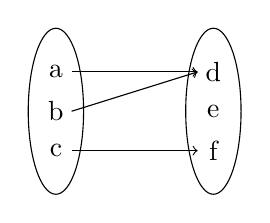
\begin{tikzpicture}
            \draw (0,0) ellipse (10pt and 30pt);
            \draw (2,0) ellipse (10pt and 30pt);

            \draw node at (0, 0.5) {a};
            \draw node at (0, 0) {b};
            \draw node at (0, -0.5) {c};

            \draw node at (2, 0.5) {d};
            \draw node at (2, 0) {e};
            \draw node at (2, -0.5) {f};

            \draw [->] (0 + 0.2, 0.5) -- (2 - 0.2, 0.5);
            \draw [->] (0 + 0.2, 0) -- (2 - 0.2, 0.5);
            \draw [->] (0 + 0.2, -0.5) -- (2 - 0.2, -0.5);
    \end{tikzpicture}
    \caption{Exemplo de função e seus conjuntos}
    \end{figure}

    \skipframe

    \item Na função abaixo, observe que:

    \begin{itemize}
        \item $D(f) = [-5, 3]$
        \item $Im(f) = [-2, 5]$
    \end{itemize}

    \begin{figure}
        \centering
        \begin{tikzpicture}[scale=0.6]
        \begin{axis}[xmin=-5, xmax=5, ymin=-5, ymax=5, axis lines=middle]
            \addplot[domain=-5:3]{x + 3};
        \end{axis}
        \end{tikzpicture}
        \caption{$f(x) = x + 3$}
    \end{figure}

    \skipframe

    \item Função: $f:\R \rightarrow \R \mid f(x) = x^2$:
    \begin{itemize}
        \item $D(f) = \R$
        \item $Im(f) = \R^+$
        \item $CD(f) = \R$
    \end{itemize}

    \begin{figure}
        \centering
        \begin{tikzpicture}[scale=0.6]
        \begin{axis}[xmin=-5, xmax=5, ymin=-5, ymax=5, axis lines=middle]
            \addplot{x^2};
        \end{axis}
        \end{tikzpicture}
        \caption{$f(x) = x^2$}
    \end{figure}

    \skipframe

    \item Função: $f:\R^+ \rightarrow \R \mid f(x) = \sqrt{x}$:
    \begin{itemize}
        \item $D(f) = \R^+$
        \item $Im(f) = \R^+$
        \item $CD(f) = \R$
    \end{itemize}

    \begin{figure}
        \centering
        \begin{tikzpicture}[scale=0.6]
        \begin{axis}[xmin=-5, xmax=5, ymin=-5, ymax=5, axis lines=middle]
            \addplot{sqrt(x)};
        \end{axis}
        \end{tikzpicture}
        \caption{$f(x) = \sqrt{x}$}
    \end{figure}

    \skipframe

    \item Função: $f:\R^* \rightarrow \R \mid f(x) = 1/x$:
    \begin{itemize}
        \item $D(f) = \R^*$
        \item $Im(f) = \R^*$
        \item $CD(f) = \R$
    \end{itemize}

    \begin{figure}
        \centering
        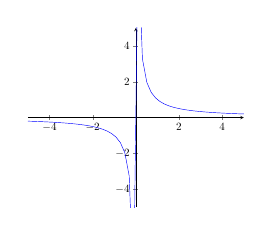
\begin{tikzpicture}[scale=0.4]
        \begin{axis}[xmin=-5, xmax=5, ymin=-5, ymax=5, axis lines=middle]
            \addplot[color=blue, samples=50]{1/x};
        \end{axis}
        \end{tikzpicture}
        \caption{$f(x) = 1/x$}
    \end{figure}

    
    
\end{itemize}
    
\end{frame}
\input{secoes/02-translacao}
\section{Funções compostas}

\begin{frame}[allowframebreaks]{Funções compostas}

\begin{itemize}
    \item Suponha que alguns valores de uma função $f$ estejam no domínio de uma função $g$. Pode-se então combinar $f$ e $g$ para formar uma nova função de $x$ e cujos valores são os números $g(f(x))$ (lê-se "$g$ de $f$ de $x$").

    \item Essa função, $g(f(x))$, é a composta de $g$ e $f$, tendo como notação $g \circ f$.

    \begin{figure}
        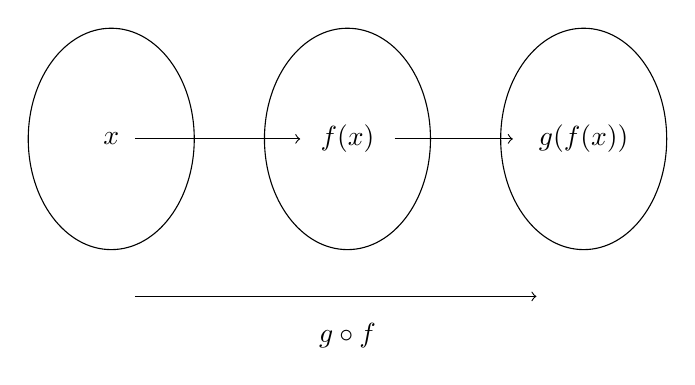
\begin{tikzpicture}
            \draw (0,0) ellipse (30pt and 40pt);
            \draw (3,0) ellipse (30pt and 40pt);
            \draw (6,0) ellipse (30pt and 40pt);

            \draw node at (0, 0) {$x$};
            \draw node at (3, 0) {$f(x)$};
            \draw node at (6, 0) {$g(f(x))$};

            \draw [->] (0 + 0.3, 0) -- (3 - 0.6, 0);
            \draw [->] (3 + 0.6, 0) -- (6 - 0.9, 0);

            \draw node at (3, -2.5) {$g \circ f$};
            \draw [->] (0 + 0.3, -2) -- (6 - 0.6, -2);
        \end{tikzpicture}
    \caption{Diagrama de composição das funções $g$ e $f$}
    \end{figure}

    \skipframe

    \item A função composta $g \circ f$ só está definida quando o contradomínio de $f$ é igual ao domínio de $g$. 
    
    \item Em geral, $g \circ f \neq f \circ g$.

    \item Pode acontecer que uma das funções $g \circ f$ ou $f \circ g$ não esteja definida.

    \skipframe

    \begin{ex}[Vendo uma função como uma composição]
        A função $y = \sqrt{1 - x^2}$ é a composição da função $g(x) = 1 - x^2$ com a função $f(x) = \sqrt{x}$. Ela pode ser pensada calculando-se primeiro $1 - x^2$ e depois tornando a raiz quadrada do resultado. Note que $1 - x^2$ não pode ser negativa. O domínio da composição é $[-1, 1]$.
    \end{ex}

    \skipframe

    \begin{ex}[Encontrando uma fórmula para a função composta]
        \emph{Dado $g(x) = x^2$ e $f(x) = x - 7$. Qual o valor de $f(g(2))$?} 

        \vspace{0.5cm}

        \textbf{R:} Para encontrar $f(g(x))$, substitui-se $x$ na fórmula $f(x) = x - 7$ pela expressão dada para $g(x)$: $f(g(x)) = g(x) - 7 = x^2 - 7 \Rightarrow f(g(2)) = 2^2 - 7 = -3$
        
    \end{ex}

    
\end{itemize}
    
\end{frame}
\section{Funções sobrejetoras, injetoras e bijetoras}

\begin{frame}[allowframebreaks]{Funções sobrejetoras}
    \begin{itemize}
        \item Uma função $f: A \rightarrow B$ é sobrejetora se, e somente se, $Im(f) = B$.

        \item Formalmente têm-se, dado que $f$ é uma função, $f: A \rightarrow B$ é sobrejetora se, e somente se, $\forall y \in B$, $\exists x \in A \mid f(x) = y$.

        \begin{multicols}{2}
            \begin{figure}
            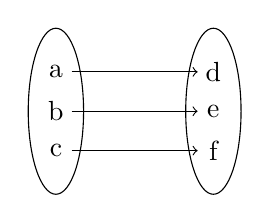
\begin{tikzpicture}
                \draw (0,0) ellipse (10pt and 30pt);
                \draw (2,0) ellipse (10pt and 30pt);
    
                \draw node at (0, 0.5) {a};
                \draw node at (0, 0) {b};
                \draw node at (0, -0.5) {c};
    
                \draw node at (2, 0.5) {d};
                \draw node at (2, 0) {e};
                \draw node at (2, -0.5) {f};
    
                \draw [->] (0 + 0.2, 0.5) -- (2 - 0.2, 0.5);
                \draw [->] (0 + 0.2, 0) -- (2 - 0.2, 0);
                \draw [->] (0 + 0.2, -0.5) -- (2 - 0.2, -0.5);
            \end{tikzpicture}
            \caption{É sobrejetora}
            \end{figure}

            \begin{figure}
            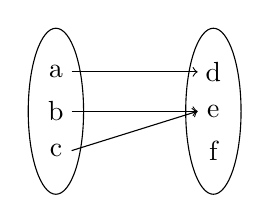
\begin{tikzpicture}
                \draw (0,0) ellipse (10pt and 30pt);
                \draw (2,0) ellipse (10pt and 30pt);
    
                \draw node at (0, 0.5) {a};
                \draw node at (0, 0) {b};
                \draw node at (0, -0.5) {c};
    
                \draw node at (2, 0.5) {d};
                \draw node at (2, 0) {e};
                \draw node at (2, -0.5) {f};
    
                \draw [->] (0 + 0.2, 0.5) -- (2 - 0.2, 0.5);
                \draw [->] (0 + 0.2, 0) -- (2 - 0.2, 0);
                \draw [->] (0 + 0.2, -0.5) -- (2 - 0.2, 0);
            \end{tikzpicture}
            \caption{Não é sobrejetora}
            \end{figure}
        \end{multicols}
    \end{itemize}
\end{frame}

\begin{frame}[allowframebreaks]{Funções injetoras}
    \begin{itemize}
        \item Uma função $f: A \rightarrow B$ é injetora se, e somente se, cada $x$ encontra um $y$ e os elementos distintos possuem imagens distintas.

        \item Formalmente têm-se, dado que $f$ é uma função, $f: A \rightarrow B$ é injetora se, e somente se, $\forall x_1, x_2 \in A, f(x_1) = f(x_2) \Rightarrow x_1 = x_ 2$.

        \begin{multicols}{2}
            \begin{figure}
            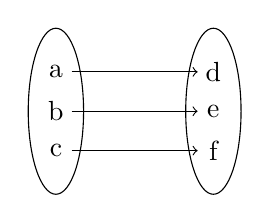
\begin{tikzpicture}
                \draw (0,0) ellipse (10pt and 30pt);
                \draw (2,0) ellipse (10pt and 30pt);
    
                \draw node at (0, 0.5) {a};
                \draw node at (0, 0) {b};
                \draw node at (0, -0.5) {c};
    
                \draw node at (2, 0.5) {d};
                \draw node at (2, 0) {e};
                \draw node at (2, -0.5) {f};
    
                \draw [->] (0 + 0.2, 0.5) -- (2 - 0.2, 0.5);
                \draw [->] (0 + 0.2, 0) -- (2 - 0.2, 0);
                \draw [->] (0 + 0.2, -0.5) -- (2 - 0.2, -0.5);
            \end{tikzpicture}
            \caption{É injetora}
            \end{figure}

            \begin{figure}
            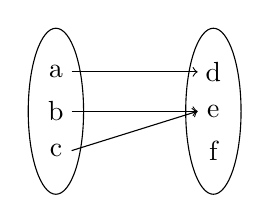
\begin{tikzpicture}
                \draw (0,0) ellipse (10pt and 30pt);
                \draw (2,0) ellipse (10pt and 30pt);
    
                \draw node at (0, 0.5) {a};
                \draw node at (0, 0) {b};
                \draw node at (0, -0.5) {c};
    
                \draw node at (2, 0.5) {d};
                \draw node at (2, 0) {e};
                \draw node at (2, -0.5) {f};
    
                \draw [->] (0 + 0.2, 0.5) -- (2 - 0.2, 0.5);
                \draw [->] (0 + 0.2, 0) -- (2 - 0.2, 0);
                \draw [->] (0 + 0.2, -0.5) -- (2 - 0.2, 0);
            \end{tikzpicture}
            \caption{Não é injetora}
            \end{figure}
        \end{multicols}
    \end{itemize}
\end{frame}
\input{secoes/05-funcoesInversas}
\input{secoes/06-funcoesPolinomiais}
\input{secoes/07-funcoesRacionais}
\input{secoes/08-funcoesAlgebricas}
\input{secoes/09-funcoesTranscendentais}
\input{secoes/10-exercicios}
\section{Respostas dos exercícios}

\begin{frame}[allowframebreaks]{Respostas dos exercícios}
    \begin{enumerate}
        \item São funções: $c$ e $d$.
        
        \item São funções: $a, d$ e $e$.
        
        \item 
        \begin{enumerate}[a]
            \item $-(x-1)$
            \item $-2x-h+2$
        \end{enumerate}

        \item 
        \begin{enumerate}[a]
            \item $D(f) = \conj{-3, -2, -1, 0, 1, 2, 3}$ e $Im(f) = \conj{1, 2, 3, 4, 5}$
            \item $D(f) = [-2, 3]$ e $Im(f) = [-3, 2]$
            \item $D(f) = [-2, 4]$ e $Im(f) = [1, 5]$
            \item $D(f) = [-3, 5)$ e $Im(f) = [1, 3)$
            \item $D(f) = [-4, 4]$ e $Im(f) = [-3, 5]$
            \item $D(f) = [-3, 4)$ e $Im(f) = \conj{-3, -2, -1, 0, 1, 2, 3}$
        \end{enumerate}

        \vspace{1cm}

        \item $D(f) = \R$ e $Im(f) = {-3}$

        \begin{figure}
        \centering
        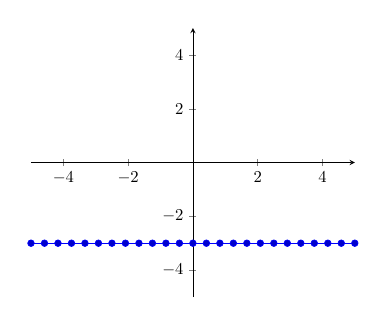
\begin{tikzpicture}[scale=0.6]
        \begin{axis}[xmin=-5, xmax=5, ymin=-5, ymax=5, axis lines=middle]
            \addplot{-3};
        \end{axis}
        \end{tikzpicture}
        \caption{$f(x) = -3$}
        \end{figure}

        \skipframe

        \item $D(f) = \R$ e $Im(f) = [0, \infty)$

        \begin{figure}
        \centering
        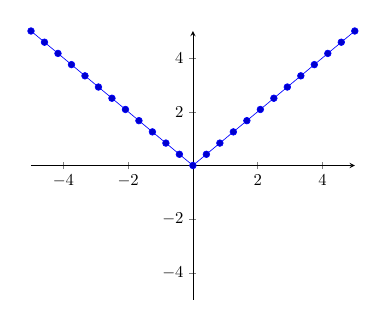
\begin{tikzpicture}[scale=0.6]
        \begin{axis}[xmin=-5, xmax=5, ymin=-5, ymax=5, axis lines=middle]
            \addplot{abs(x)};
        \end{axis}
        \end{tikzpicture}
        \caption{$f(x) = \abs{x}$}
        \end{figure}

        \item <colocar gráficos>

        \skipframe

        \item $D(f) = [-2, 6)$ e $Im(f) = [-2, 4]$

        \item $D(f) = [3, \infty) - {5}$

        \item $(1/2, \infty)$

        \skipframe

        \item $D(f) = (-\infty, \infty) - {5}$ e $Im(f) = [-1, \infty)$. O gráfico de $f$ corresponde ao do valor absoluto deslocado duas unidades para a direita e uma unidade verticalmente.

        \vspace{0.5cm}

        \begin{figure}
        \centering
        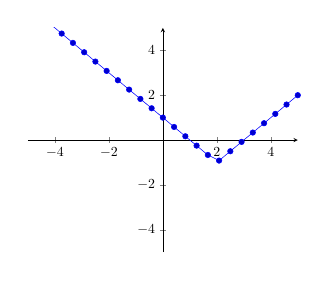
\begin{tikzpicture}[scale=0.5]
        \begin{axis}[xmin=-5, xmax=5, ymin=-5, ymax=5, axis lines=middle]
            \addplot{abs(x-2)-1};
        \end{axis}
        \end{tikzpicture}
        \caption{$f(x) = \abs{x-2}-1$}
        \end{figure}

        \skipframe

        \item 
        \begin{enumerate}[a]
            \item Posição 4.
            \item Posição 1.
            \item Posição 2.
            \item Posição 3.
        \end{enumerate}
    \end{enumerate}
\end{frame}

\end{document}